\subsection{Shape from Shading}

The depth camera measures IR reflectance in addition to depth at each pixel.  Since the reflectance depends on the angle between the surface normal and the incident ray from the IR illuminator, the reflectance image can provide useful cues on the object surface.  Shape from shading techniques model this dependence on the surface normal, along with additional surface assumptions such as smoothness, to estimate the normals and integrate an object surface [REF].  However the real world practicality of these methods has been limited since they generally require a single known light source position illuminating a Lambertian surface, the integration is sensitive to noise, and shape is obtained only up to a scale factor.  Fortunately our application satisfies the key requirements of Shape from Shading, (we have a known light source and leafs are modeled well as Lambertian surfaces~\cite{Chelle2006219}), and our mesh model provides additional information that removes the need to integrate noisy surface normals.  This section describes our use of Shape from Shading to improve shape recovery.

\begin{figure}
\begin{center}
   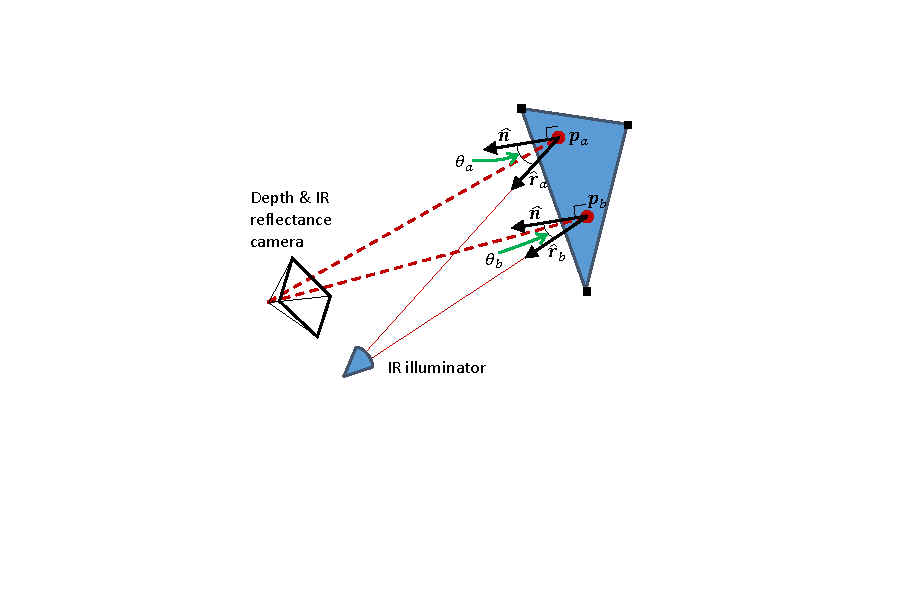
\includegraphics[trim=100 100 100 40,clip,width=0.95\linewidth]{Figures/ShapeFromShading}
\end{center}
   \caption{Our geometric model for the reflectance image.  At each depth point the intensity of the reflectance image will depend on a number of factors including the angle between the facet normal and the ray to the illuminator shown for two points as $\theta_a$ and $\theta_b$. }
\label{fig:shapefromshading}
\end{figure}

\subsubsection{Reflectance Modeling}

We build a simplified bidirectional reflectance model to explain the pixel values, $R_i$, of the IR reflectance image, shown in Figure~\ref{fig:plantnoise}($b$).  This model for pixel $i$ is:
\beq
R_i = \frac{I_i\rho \ray_i\cdot\normal_i s_i}{r_i^2}.\label{eq:reflectanceinit}
\eeq
Here $I_i$ is the intensity of the ray from the IR illuminator assumed to be a point source and decreasing with the inverse square of the distance to target, $r$. Under a Lambertian assumption the reflected beam is decreased by the albedo, $\rho$, and the inner product of the unit ray direction $\ray_i$ and the unit normal, $\normal_i$.  Finally the sensor scales the incoming beam with a factor $s_i$.  This model can be simplified further by approximating the outgoing ray $I_i$ as being the same for a given pixel regardless of target depth.  We define a pixel gain $g_i = \log(I_i s_i)$, and the resulting model is:
\beq
R_i = \frac{ \rho \exp(g_i) \ray_i\cdot\normal_i }{r_i^2}. \label{eq:reflectance}
\eeq

The gain values can be calculated from a single depth image of a known surface with constant albedo up to a scale factor (of the unknown albedo).  We observe large gain near the center of the image with tapering towards the edges, along with inter-pixel variations.  We chose to treat the pixel variations as noise and model the gain as a polynomial in normalized pixel coordinates, $u$ and $v$.  That is our modeled gain is:
\beq
g(u,v) = \beta_1 + \beta_2 u + \beta_3 v + \beta_4 u^2 + \beta_5 v^2 \label{eq:gainmodel}
\eeq
Taking the $\log$ of Eq.~(\ref{eq:reflectance}) we can do a least squares fit of the parameters $\beta_i$ and so characterize the gain.  We used a flat target with constant albedo and took data at various inclinations and depths. Figure~\ref{fig:gain} shows the resulting gain model, along with data from one depth image.   

\begin{figure}
\begin{center}
   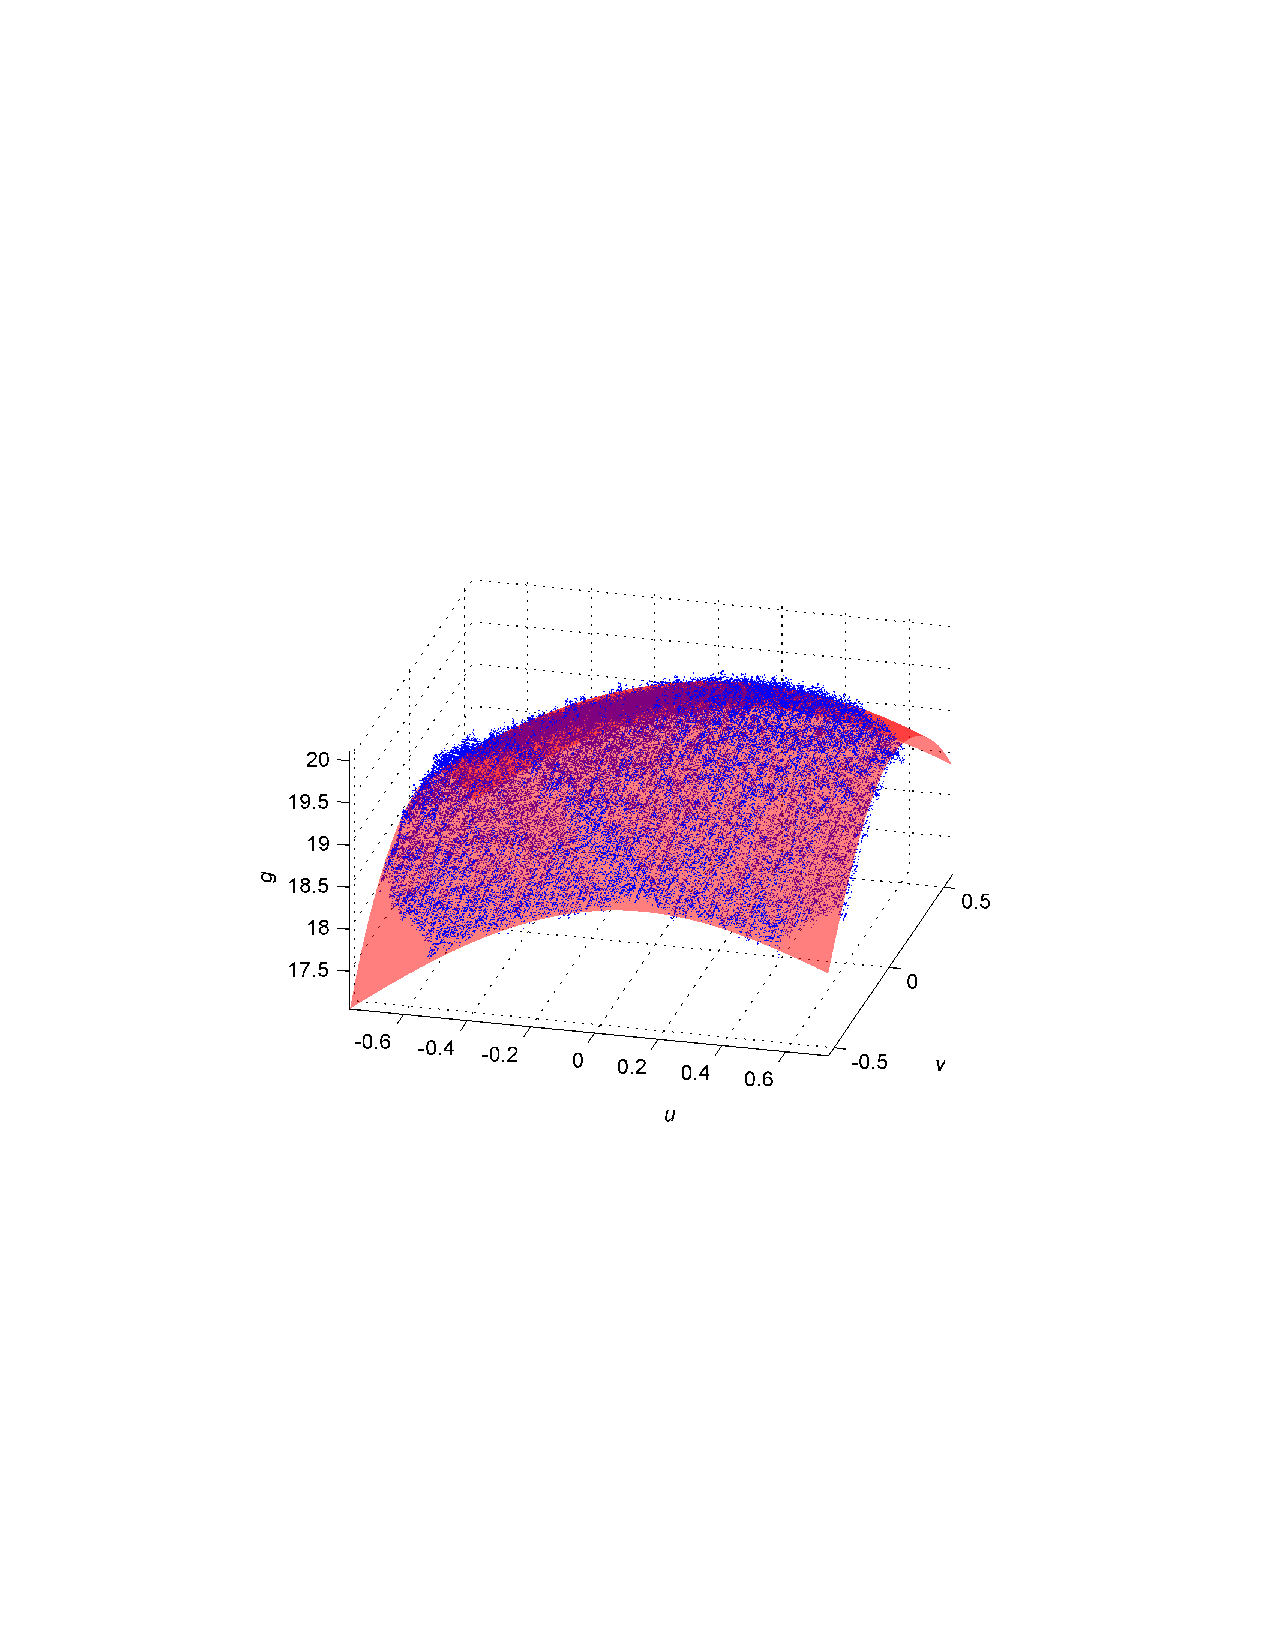
\includegraphics[trim=100 250 100 250,clip,width=0.95\linewidth]{Figures/gain}
\end{center}
   \caption{Our model for gain $g(u,v)$ in Eq, (\ref{eq:gainmodel}) is fit to a $\log$ reflectance image adjusted with known range and ray angles from Eq.~(\ref{eq:reflectance}).  The dots are the measured data and the surface is the parameterized gain $g(u,v)$. }
\label{fig:gain}
\end{figure}


\subsubsection{Mesh Normals Estimation}

Given a reflectance image providing, $R_i$ for each pixel, a depth image from which we can calculate range to each pixel, $r_i$, and our gain model, $g(u,v)$, we can rearrange and Eq.~({eq:reflectance}) to obtain an inclination prediction, $\eta_i$ at each pixel:
\beq
\eta_i \equiv \rho_t\cos(\theta_i) = R_ir_i^2\exp(-g(u,v)). \label{eq:costheta}
\eeq
The scale factor is the unknown target albedo, $\rho_t$.  If the target such as a leaf has a uniform albedo, this is the same for all target pixels.  

Now each mesh facet has a unit normal which can be encoded in terms of the depths of its three vertices: $\normal(\lambda_a,\lambda_b,\lambda_c)$.  The inner product of this normal with the unit ray to the illuminator is $\cos(\theta)$ and should agree with the values predicted in Eq. (\ref{eq:costheta}) for each reflectance pixel it contains.  This leads to a Shape from Shading cost of
\beq
E_{SfS}(\vlambda_v, \rho_t) = \sum_{i\in \mathcal{T}}\| \frac{\eta_i}{\rho_t} - \normal_i\cdot\ray_i \|^2.
\label{eq:esfs}
\eeq
The sum is over all target pixels, $\mathcal{T}$, projecting into the image mesh, and $\normal_i$ indicates the normal of the facet into whose image the depth pixel projects.  This cost introduces the unknown target albedo, $\rho_t$, as an addition parameter to be optimized over.  The cost is nonlinear, but given a good initial parameters from the least squares solution to Eq.~(\ref{eq:meshleastsquares}), it is readily minimized as a function of vertex depths and albedo.
